\documentclass{report}

\usepackage[francais]{babel}
\usepackage[latin1]{inputenc}
\usepackage{xspace}
\usepackage{float}
%\usepackage{here}
\usepackage{geometry}
\usepackage[dvips]{graphicx}
\usepackage[pdftex,
  colorlinks=true,
  pdfstartview=FitV,
  linkcolor=blue,
  citecolor=blue,
  urlcolor=blue]{hyperref}
  
\newcommand{\visidia}{ViSiDiA\xspace}
\newcommand{\berlios}{BerliOs.de\xspace}
\newcommand{\labri}{LaBRI\xspace}

\author{}
\date{}

\title{
  \begin{flushright}
    \begin{Huge}
      \begin{textbf}
        Projet \visidia\\
      \end{textbf}
    \end{Huge}
    \rule{\textwidth}{2mm}\\
    \large\rm{Rapport}\\
    \vspace{2cm}
    \begin{textbf}\\
      \underline{Auteurs}~:\\
      \vspace{0.5cm}
      \sc
      Ammar Aymen\\
      Balan Alexandre\\
      Ben Alaya Ramzi\\
      Bochu Fabien\\
      Bonin �ric\\
      Lafon Julien\\
      \vspace{5mm}
    \end{textbf}
    \rm 6 avril 2007\\
    \vspace{6.25cm}
  \end{flushright}
  \begin{flushleft}
    %\rule{\textwidth}{2mm}\\
    \small
    \underline{Responsable p�dagogique}~: David Renault.\\
    \underline{Responsables scientifiques}~: Mohamed Mosbah et Brahim Hamid.
  \end{flushleft}
}

\begin{document}


\maketitle
\tableofcontents

\chapter*{Introduction}
\addcontentsline{toc}{chapter}{Introduction}
\chapter*{Introduction}
%          * D�crire la probl�matique et la motivation
%          * Placer le syst�me dans son contexte
%          * Donner son r�le dans l'organisation qui l'englobe 


\subsection*{Contexte d'utilisation}

L'algorithmique distribu�e devient de nos jours de plus en plus
importante aux vues des utilisations possibles sur les r�seaux et
autres syst�mes distribu�s.%\\

Cependant,  les   applications  distribu�es  qui   en  d�coulent  sont
difficiles � implanter, tester  et exp�rimenter.  En effet, celles-ci,
en  plus  des  probl�mes  des  applications  classiques  centralis�es,
doivent  g�rer  des probl�mes  de communication  entre processus,  de
concurrence  et de  conflits  de  ressources.  C'est  dans  le but  de
faciliter la t�che � un d�veloppeur d'algorithmes  distribu�s que des
chercheurs  du  LaBRI  ont   cr��  \visidia.%\\

Ce logiciel est un atelier proposant des outils
de simulation  et  de visualisation,  au travers  d'animations 
graphiques en temps r�el, de l'ex�cution d'un algorithme distribu� sur
un graphe  donn�.  Cet algorithme peut �tre  choisi dans une liste,
algorithme d�velopp� par  l'utilisateur ou encore  dessin� gr�ce � des
r�gles de r��criture.%\\ 

L'application  va  donc  constituer  �  terme un  outil permettant la 
validation pratique de r�sultats th�oriques sur un environnement
distribu�.
\subsection*{D�finition d'un r�seau}

Un r�seau est un graphe dont les sommets sont les processeurs et les
ar�tes sont les liens de communication.%\\  

\subsection*{Notions d'algorithmique distribu�e}

Il existe de nombreux mod�les permettant de d�crire des algorithmes
distribu�s. Parmi eux, deux ont �t� d�velopp�s dans \visidia : la
communication par 
�change de message et par agent.%\\ 

Dans la suite, nous parlerons de m�moire d'un agent et d'un sommet
mais la m�moire d'un sommet contient le whiteboard et l'�tat de ses
ports.%\\ 

\subsubsection*{Communication par message}

Dans ce mod�le, chaque n\oe ud repr�sente un syst�me ou un processeur. Sur chaque
n\oe ud est ex�cut� un algorithme disposant de certaines primitives qui lui permettent de
communiquer � l'aide de messages avec ses n\oe uds voisins.
Les n\oe uds sont reli�s entre eux par des canaux de communication
(les ar�tes du graphe) par lesquels transitent les messages. 

\subsubsection*{Communication par agent} (??? a modifier)

Ce second mod�le, plus r�cent que le pr�c�dent, consid�re que le syst�me
repr�sent� par un n\oe ud ne dispose pas d'unit� de calcul mais seulement d'une
m�moire. Les n\oe uds sont ainsi d�pourvu d'algorithme et ne peuvent donc pas
communiquer directement entre eux.%\\

L'ex�cution des algorithmes se fait par des agents. Ces entit�s poss�dent une
capacit� de calcul ainsi qu'une m�moire. Un agent se d�place dans le graphe
et ex�cute un algorithme qui lui est associ�.


\subsection*{L'existant}

\visidia impl�mente aujourd'hui les deux mod�les de communication pr�sent�s
pr�c�demment. La gestion des agents a �t� ajout�e l'ann�e derni�re. Seule cette
partie concernera le projet, la partie sur la communication par message ne sera
pas �tudi�e.%\\

L'application \visidia a �t� r�alis�e en respectant une s�paration en
trois parties, interface graphique, simulateur et algorithmes. 
L'interface graphique permet � l'utilisateur d'interagir avec le
programme et de consulter l'avancement d'une ex�cution d'agent sur un
graphe. Elle est synchronis�e avec le simulateur pour �viter toute
incoh�rence. Elle fournit quelques statistiques de base sur
l'ex�cution. Le simulateur coordonne les op�rations. C'est le c\oe ur
de \visidia. Enfin, ce sont les agents  qui vont r�aliser ces
op�rations sur le graphe.%\\ 

Une biblioth�que  de primitives de  base (\emph{API}) est mise �
disposition de l'utilisateur afin qu'il puisse r�aliser ses propres
algorithmes � base d'agent. 


\subsection*{Motivations et but}

La version avec agent mobile de \visidia offre aujourd'hui suffisamment de
fonctionnalit�s pour simuler les algorithmes � base d'agent mobile.%\\

N�anmoins, contrairement � la partie de \visidia avec communication par message
qui poss�de un grand nombre d'algorithmes d�velopp�s, la partie avec agent mobile
se limite � quelques-uns. L'impl�mentation des algorithmes dans \visidia n'est
pas ais�e et la proc�dure est peu document�e, le client a donc besoin
que les algorithmes soient impl�ment�s pour lui.%\\ 

Les statistiques sur l'ex�cution des algorithmes est un point particuli�rement
important pour le client. En effet, \visidia est un outil qui lui permet de
confronter r�sultats th�oriques et exp�rimentaux. C'est les statistiques qui
permettent cette comparaison et celles-ci sont actuellement tr�s limit�es.%\\

Un autre besoin du client est de pouvoir agir sur le graphe au cours de
l'ex�cution d'un algorithme. En effet, en algorithmique distribu�e on
s'int�resse aux cons�quences d'une �volution de la topologie du r�seau, de
l'alt�ration des m�moires d'un n\oe ud du r�seau ou d'un agent, voire du crash
accidentel d'un de ces derniers.


\chapter{Domaine d'application}
\visidia est une application de simulation d'ex�cution d'algorithmes distribu�s.
Pour une bonne compr�hension de ce rapport, nous allons vous pr�senter les
principes de l'algorithmique distribu�.

\section{Pr�sentation de l'algorithmique distribu�e}

\subsection{D�finition}
Tout algorithme distribu� s'ex�cute sur un r�seau. Un r�seau pouvant �tre
mod�lis� par un graphe o� les sommets repr�sentent les entit�s(machines ou processeurs)
voulant communiquer entre elles et les ar�tes repr�sentent un canal de
communication (connexion) entre deux entit�s. 
%Remarque : Un arc entre deux entit�s signifie que la communication ne peut
%s'effectuer que dans un sens.
\begin{figure}[ht]
  \centering
  \includegraphics[width=5cm,height=5cm]{images/graphe.png}
  \caption{Exemple de mod�lisation d'un syst�me distribu�}
\end{figure}


\subsection{Communication et Syst�me distribu�}
Dans un syst�me distribu�, la communication peut s'effectuer selon deux modes :
\begin{itemize}
  \item le mode synchrone o� le temps est une donn�e globale du
    r�seau, c'est-�-dire que les (blocs d') instructions de
    l'algorithme s'effectuent sur les tops de l'horloge~;
  \item le mode asynchrone o� les op�rations peuvent se produire �
    n'importe quel instant ind�pendemment de l'ex�cution de celle des
    autres agents.
\end{itemize}

\begin{figure}[ht]
  \centering
  \includegraphics[width=8cm]{images/algodist.png}
  \caption{Les  types  des r�seaux  en  terme  de synchronisation,  un
  sch�ma similaire peut �tre �labor� en s'appuyant sur la connaissance
  ou non des noeuds du r�seau}
  \label{fig:algodist}
\end{figure}

\subsection{Les deux mod�les d'algorithmes}
Il existe deux mod�les d'algorithmes distribu�s :
\begin{itemize}
  \item le mod�le par envoi de messages o� chaque entit�s dispose d'un algorithme qu'elle
  ex�cute et communique avec ses entit�s voisines par l'envoi de message sur le
  r�seau~;
  \item le mod�le avec agent o� les entit�s sont passives, c'est-�-dire
    qu'elles n'effectuent pas de traitement de leur propre initiative,
    les algorithmes sont contenus dans des agents mobiles, qui sont
    des �l�ments poss�dant un algorithme et une m�moire, qui se
    d�placent sur le r�seau et utilisent les sites passifs et leur m�moire pour
    ex�cuter leur algorithme. 
\end{itemize}


\section{Exemple d'algorithmes distribu�e}

Dans le  domaine de l'algorithmique distribu�e,  de nombreux probl�mes
existent, en voici quelques uns des plus fr�quent.

\subsection{Le probl�me de l'�lection}
Ce probl�me consiste � distinguer une entit� c'est-�-dire de
l'�lire. La plupart du temps cette �lection permet de s�lectionner une
entit�e pour lui permettre d'acc�der � une ressource critique, les
entit�es non-�lues n'y ayant pas acc�s.

\subsection{D�tection de la terminaison}
La d�tection de la terminaison d'un algorithme distribu� est souvent difficile,
car elle n�cessite pas seulement d'avoir la connaissance de la terminaison de
son algorithme mais �galement de celle de tous les entit�s  du r�seau.
Nous pouvons cependant chercher �  avoir un d�tection locale de  la terminaison
globale, c'est-�-dire qu'un processeur  peut savoir en fonction de  son �tat et
de celui de ces voisins si l'algorithme est termin�.

\section{Quelques applications}



\chapter{Analyse de l'existant}
\section{Pr�sentation de \visidia}

\subsection{L'application}

Avec la g�n�ralisation des r�seaux tels qu'Internet et le d�veloppement d'une
information de plus en plus complexe et massivement distribu�e sur ces grands
r�seaux, de nombreuses applications industrielles, bancaires et Web sont elles
aussi devenues distribu�es.

Toutefois, le d�veloppement d'applications distribu�es est un processus tr�s difficile.
� la complexit� classique de d�veloppement d'applications centralis�es, s'ajoute une complexit� 
li�e � la distribution et � l'introduction de la communication entre processus, de la concurrence,
des conflits de ressources. 

C'est dans ce cadre, que les chercheurs du LaBRI ont lanc� le projet
ViSiDiA\footnote{\url{http://www.labri.fr/projet/visidia}}. 
\visidia se propose de fournir un atelier compos� d'outils de simulation, de
visualisation et d'aide aux preuves devenus indispensables pour la conception,
les tests et la validation de programmes dans des environnements distribu�s. Le mod�le
classique consiste � repr�senter le r�seau par un graphe o� les 
sommets correspondent � des machines ou processeurs, et les ar�tes � des
connexions.

\visidia impl�mente les deux mod�les d'algorithmes distribu�s, la version avec
envoi de messages, et celle � base d'agents mobiles.
Nous nous int�ressons seulement � la simulation avec les agents mobiles
durant ce projet.

\subsection{Architecture g�n�rale}

Nous allons maintenant nous attarder � d�crire l'architecture g�n�rale
du programme \visidia dans sa version avec agents mobiles.

\visidia se base sur trois grandes structures~:

\begin{itemize}

\item l'interface graphique ;
\item le simulateur ;
\item les agents.

\end{itemize}

\begin{figure}[H]
  \centering
  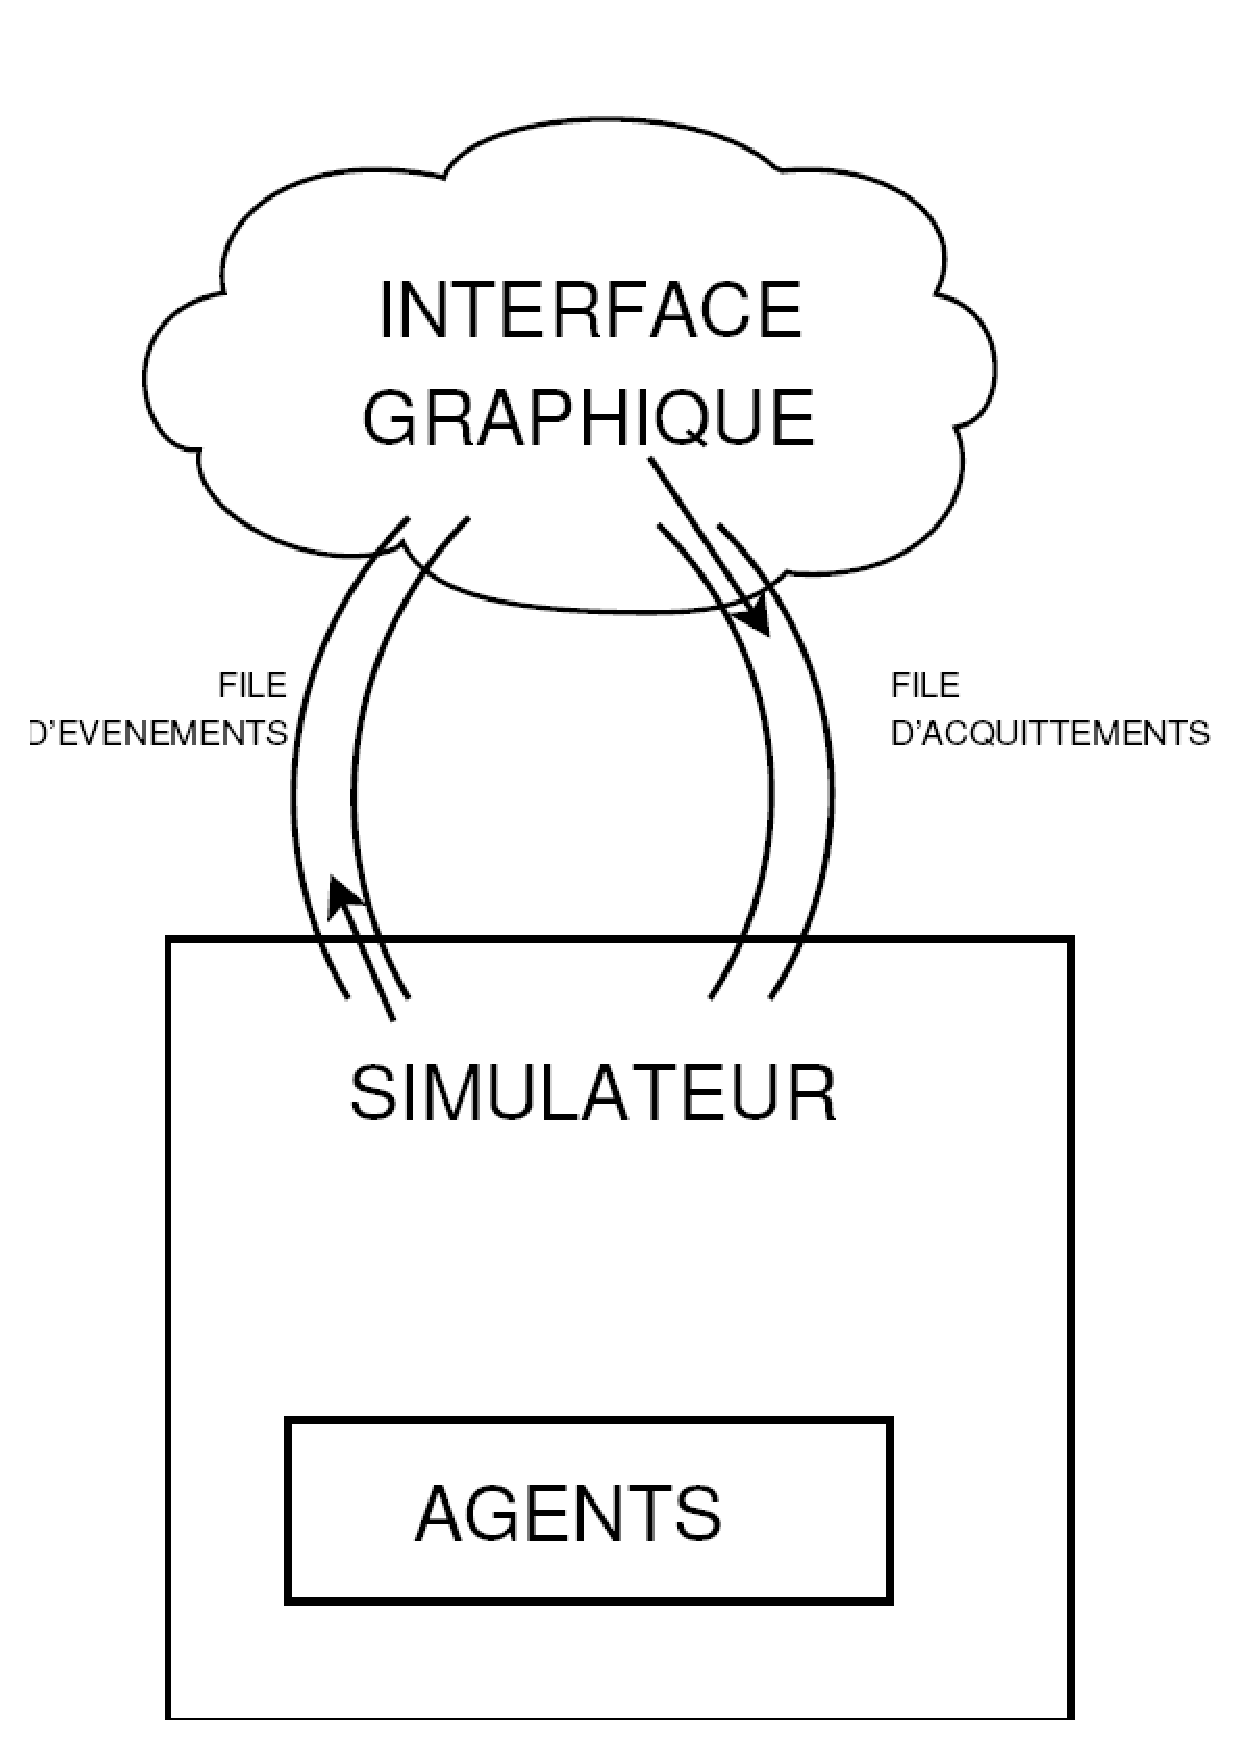
\includegraphics[width=6cm]{images/structureVisidia.png}
  \caption{Structuration de \visidia}
  \label{fig:implantation-communication}
\end{figure}


\subsubsection{Interface graphique}

L'interface graphique est une  partie tr�s importante de l'application
\visidia. C'est  gr�ce �  elle que \visidia  a beaucoup de  succ�s. En
effet,  elle permet  de visualiser  en temps  r�el le  d�placement des
agents sur le graphe et l'�tat des sommets.

L'interface graphique se compose de  deux parties : la premi�re partie
est  consacr�e � l'�dition  de graphe  et la  seconde �  la simulation
proprement dite.

\paragraph{Interface graphique d'�dition}

\begin{figure}[ht]
  \centering
  \includegraphics[width=10cm]{images/existant-edition.png}
  \caption{Ecran principal de \visidia :  un graphe est dessin�}
  \label{fig:existant-edition}
\end{figure}

Dans la partie consacr�e  � l'�dition, l'interface graphique permet de
cr�er de nouveaux graphes par la seule utilisation de la souris. Gr�ce
� elle, de simples glisser/d�poser permettent de placer des sommets et
de les relier par des ar�tes.

Cette interface permet aussi de  charger des graphes existants, de les
compl�ter\dots

\paragraph{Interface graphique de simulation}

\begin{figure}[ht]
  \centering
  \includegraphics[width=10cm]{images/existant-simulation.png}
  \caption{Algorithme de simulation avec agent en cours d'ex�cution.}
  \label{fig:existant-simulation}
\end{figure}

La partie la plus int�ressante de l'interface graphique se trouve dans
la fen�tre de simulation. De nombreuses t�ches peuvent �tre effectu�es
dans cette partie parmi lesquelles~:

\begin{itemize}

\item charger un algorithme et le placer sur les sommets du graphe ;
\item lancer la simulation, la mettre en pause et l'arr�ter ;
\item voir en temps r�el les agents circuler sur les ar�tes ;
\item choisir des r�gles de r��criture � appliquer ;
\item �diter les �tiquettes des sommets.

\end{itemize}

\subsubsection{Simulateur}

Le simulateur est  le noyau de \visidia. Il a  entre autre pour charge
de~:

\begin{itemize}
\item g�rer les agents du r�seau ;
\item informer l'interface graphique des changements ;
\item valider les acquittements de l'interface graphique ;
\item compter les �v�nements en vue d'�tablir des statistiques.\\
\end{itemize}

Lorsque le simulateur est cr�� par l'interface graphique, celle-ci lui
fournit  le  graphe  courant,  les agents choisis  par
l'utilisateur  et deux files  qui serviront  � la  communication (voir
\ref{sec:existant-communication}). Le simulateur se charge � ce moment
d'initialiser les  files de messages pour les  agents. Mais c'est
au moment  o� le  simulateur re�oit un  appel �  $startSimulation$ que
celui-ci commence  r�ellement son travail.   Il va cr�er,  pour chaque
agent, un processus  qui va ex�cuter le code de l'algorithme
lorsqu'un agent est sur un sommet.

Par la  suite, le r�le  du simulateur sera  de g�rer les  demandes des
agents et de l'interface graphique (mise en pause ou � l'arr�t
du simulateur\dots).

\subsubsection{Les agents}

Les agents repr�sentent la  partie �volutive de \visidia. Pour se
servir  de  \visidia,  l'utilisateur  devra commencer  par  �crire  un
algorithme en Java  en utilisant l'API fournie (il  est aussi possible
de dessiner  des r�gles  de r��critures).

Lors   du   lancement  de   la simulation,   la   m�thode  $init$ de chaque 
agent est appel�e.  C'est  cette  m�thode  que l'utilisateur  de  \visidia  doit
impl�menter. 

Chaque  agent du  graphe va  ex�cuter sa  propre copie  de  la m�thode
$init$.


\subsubsection{Communication entre les structures}
\label{sec:existant-communication}

Dans  cette partie  nous d�crirons  bri�vement comment  les structures
communiquent    entre    elles.     

\paragraph{Entre la partie graphique et le simulateur :}

Deux    files    permettent    la
communication entre  le simulateur et l'interface  graphique. Ces deux
files  sont cr��es par  l'interface graphique  et pass�es  en param�tre
lors de la construction du simulateur.

Quand le  simulateur a besoin  de faire faire  une action �  la partie
graphique,   ou  lorsque  le   simulateur  souhaite   l'informer  d'un
�v�nement, il cr�e un nouvel objet de type $SimulEvent$ et le place
dans la file d'�v�nements. Ces �v�nements sont de plusieurs types~:

\begin{itemize}
\item changement de l'�tat d'un noeud ou d'une ar�te,
\item d�placement d'un agent,
\item nouveau round pour les agents synchronis�s
\end{itemize}

Lorsque l'interface  graphique re�oit un  �v�nement sur la  file, elle
ex�cute  les  t�ches n�cessaires  puis  elle  confirme l'ex�cution  en
envoyant  un acquittement sur  la seconde  file. Le  simulateur attend
l'acquittement  de  l'interface  graphique  avant  de  consid�rer  que
l'action  a  �t�  effectu�e.  Ceci  permet  de  garder  une  interface
graphique synchronis�e avec le simulateur.


\paragraph{Entre les agents et le simulateur :}
La communication entre les agents  et le simulateur est bien plus
classique. Chaque agent poss�de un lien direct vers le simulateur
gr�ce  � une  variable d'instance.   A  partir de  l�, faire  ex�cuter
quelque  chose au  simulateur reviens  � appeler  une  m�thode d'acc�s
publique sur cette variable.



\section{L'aspect technique}

\subsection{Code source}

Nous avons r�cup�r� la derni�re version de d�veloppement de \visidia. Celle-ci
est disponible sur notre svn : 
\begin{verbatim}
svn checkout svn://svn.berlios.de/visidia/trunk
\end{verbatim}

Le code source de \visidia est parfois comment� avec l'outil \textbf{javadoc}. 
Tr�s peu de classes et d'attributs ont �t� comment�s.

\subsection{Documentation}

La documentation qui nous a �t� fournie a �t� le rapport de
PFA de l'�quipe pr�c�dente. Nous n'avons pas eu connaissance de l'existence d'un
rapport technique
expliquant les principes techniques de d�veloppement de l'application depuis son
d�but.

\chapter{Expression du besoin}
Dans cette partie, nous allons d�crire les besoins fonctionnels li�s au projet (ajout de nouvelles fonctionnalit�s, modification de l'interface) ainsi que les besoins non fonctionnels (langage, licence, etc).

\section{Besoins fonctionnels}

Nous d�crivons ici les nouvelles fonctionnalit�s du logiciel \visidia. Nous nous attarderons simplement � d�tailler les entr�es et sorties de chaque nouvelle fonctionnalit�, sans aborder l'impl�mentation (qui fera l'objet du prochain chapitre portant sur l'impl�mentation). Les sp�cifications des besoins fonctionnels d�crivent le nouveau comportement externe du logiciel \visidia.


\subsection{Mise en pause du programme}
Cette fonctionnalit� �tait d�j� pr�sente dans le logiciel au d�but du projet : l'appui sur un bouton de mise en pause interrompt tous les agents en cours d'ex�cution. Cependant cette fonctionnalit�, n�cessaire lors d'une modification sur un agent ou sur le graphe pendant la simulation (c'est-�-dire pendant l'ex�cution), est devenue compl�tement transparente pour l'utilisateur. Ce dernier n'a pas besoin de mettre en pause le programme lors d'une modification dans la fen�tre de simulation.\\

\begin{itemize}
  \item Entr�e : modification (sur un agent ou sur le graphe) pendant la simulation
  \item Sortie : mise en pause automatique, modification apport�e, simulation toujours en cours d'ex�cution
\end{itemize}


\subsection{Modification de la m�moire d'un sommet}
Pendant l'ex�cution d'un algorithme avec agents mobiles, l'utilisateur peut modifier l'�tat de la m�moire d'un sommet. L'utilisateur s�lectionne le sommet dont il souhaite modifier la m�moire : il peut alors consulter sa m�moire puis la modifier pendant l'ex�cution de l'algorithme.\\

\begin{itemize}
  \item Entr�e : s�lection d'un sommet
  \item Sortie : apr�s consultation de l'�tat de la m�moire du sommet, modification de la m�moire du sommet
\end{itemize}


\subsection{Extinction d'un sommet}
Pendant l'ex�cution d'un algorithme avec agents mobiles, l'utilisateur peut �teindre un sommet : celui-ci fait toujours partie du graphe, mais il est \textit{�teint}. Les sommets voisins du sommet �teint n'envoient alors plus d'agents mobiles vers ce sommet tant que celui-ci ne sera pas \textit{rallum�}. Si un agent a d�j� �t� envoy� vers ce sommet �teint (lors de l'extinction, l'agent se trouve sur une ar�te incidente), alors l'agent est renvoy� vers le sommet dont il provient.\\

\begin{itemize}
  \item Entr�e : s�lection d'un sommet
  \item Sortie : sommet �teint ne traitant plus les agents
\end{itemize}


\subsection{Remise en fonctionnement d'un sommet : allumer un sommet}
Pendant l'ex�cution d'un algorithme avec agents mobiles, l'utilisateur peut allumer un sommet �teint : cette action est compl�mentaire � l'extinction d'un sommet. Un sommet �teint peut �tre rallum�, c'est-�-dire que ce sommet devient comme initialement parfaitement fonctionnel.\\

\begin{itemize}
  \item Entr�e : s�lection d'un sommet
  \item Sortie : sommet allum� traitant � nouveau les agents
\end{itemize}


\subsection{Ajout d'un sommet}
Pendant l'ex�cution d'un algorithme avec agents mobiles, l'utilisateur peut ajouter un sommet. Cette action peut s'effectuer plusieurs fois de suite, sans que le programme soit mis en pause.\\

\begin{itemize}
  \item Entr�e : s�lection d'une zone o� ajouter un sommet
  \item Sortie : sommet ajout� pendant l'ex�cution de l'algorithme
\end{itemize}


\subsection{Suppression d'un sommet}
Pendant l'ex�cution d'un algorithme avec agents mobiles, l'utilisateur peut supprimer un sommet. Toutes les ar�tes incidentes au sommet sont �galement supprim�es. Si un agent est pr�sent sur le sommet lors de la suppresion, alors l'agent est tu�. Il en vient de m�me pour les agents pr�sents sur les ar�tes supprim�es.\\

\begin{itemize}
  \item Entr�e : s�lection d'un sommet � supprimer
  \item Sortie : sommet supprim� ansi que toutes les ar�tes qui lui sont incidentes
\end{itemize}


\subsection{Ajout d'une ar�te}
Pendant l'ex�cution d'un algorithme avec agents mobiles, l'utilisateur peut ajouter une ar�te. L'ajout d'ar�te s'effectue entre deux sommets d�j� pr�sents, par un \textit{glisser-d�placer} avec clic gauche de la souris.\\

\begin{itemize}
  \item Entr�e : s�lection du premier sommet, puis \textit{glisser-d�placer} vers le second sommet
  \item Sortie : ar�te ajout�e entre les deux sommets
\end{itemize}


\subsection{Suppression d'une ar�te}
Pendant l'ex�cution d'un algorithme avec agents mobiles, l'utilisateur peut supprimer une ar�te. Il suffit de s�lectionner l'ar�te � supprimer et d'activer le bouton ad�quat. Si un agent est pr�sent sur l'ar�te en cours de suppression, celui-ci est tu�.\\

\begin{itemize}
  \item Entr�e : s�lection d'une ar�te � supprimer
  \item Sortie : ar�te supprim�e
\end{itemize}


\subsection{Ajout d'un agent}
Pendant l'ex�cution d'un algorithme avec agents mobiles, l'utilisateur peut ajouter un agent. Apr�s avoir s�lectionn� le sommet o� ajouter l'agent, l'utilisateur choisit ensuite le type d'agent qu'il souhaite ajouter.\\

\begin{itemize}
  \item Entr�e : s�lection d'un sommet o� ajouter un agent
  \item Sortie : apr�s s�lection du type d'agent, ajout de l'agent sur le sommet et ex�cution de son algorithme
\end{itemize}


\subsection{Suppression d'un agent}
Pendant l'ex�cution d'un algorithme avec agents mobiles, l'utilisateur peut supprimer un agent. L'utilisateur active le bouton permettant la suppression d'agent : il s�lectionne ensuite le nom de l'agent qu'il d�sire supprimer. Ce dernier sera alors d�finitivement supprim� de la simulation.\\

\begin{itemize}
  \item Entr�e : activation du bouton de suppression d'agents
  \item Sortie : apr�s s�lection du nom de l'agent, suppression d�finitive de l'agent dans la simulation
\end{itemize}


\subsection{Modification de la m�moire d'un agent}
Pendant l'ex�cution d'un algorithme avec agents mobiles, l'utilisateur peut modifier la m�moire d'un agent. L'utilisateur active le bouton de consultation des m�moires des agents. Apr�s avoir s�lectionn� l'agent � consulter, l'utilisateur active le bouton de modification de sa m�moire : il s�lectionne ensuite le champ � modifier et entre une nouvelle valeur.\\

\begin{itemize}
  \item Entr�e : activation du bouton de consultation de la m�moire des agents
  \item Sortie : apr�s s�lection du nom de l'agent puis du champ � modifier, la nouvelle valeur est entr�e dans la m�moire de l'agent
\end{itemize}


\subsection{Statistiques}
Pendant l'ex�cution d'un algorithme avec agents mobiles, l'utilisateur peut afficher en temps r�el des statistiques par agent et des statistiques sur l'ex�cution d'un algorithme. 


\section{Besoins non fonctionnels}

\subsection{Structuration de l'application}

\subsection{Langage et portabilit�}



\chapter{Travail r�alis�}
\section{Ajout de fonctionnalit�s}

\subsection{Modification du graphe en cours d'ex�cution}

\subsection{Structure du graphe}

Dans visidia, il y a une s�paration totale entre la partie affichage et la
partie simulation. Ainsi, \visidia manipule deux graphes : un graphe visuel et un
autre pour la simulation.\\

N'ayant aucune indication sur les structures de ces graphes, on pouvait imaginer
que les structures de ces graphes pouvaient �tre les m�mes, ou bien avoir des
points en commun.\\

Apr�s une analyse plus pouss� du code, nous avons d�couvert que les deux
structures �taient totalement dissoci�s et ind�pendante l'une de l'autre.
Pour la partie simulation, le r�pertoire ``graph'' contient toutes les classes
de l'architecture du graphe.
%inclure sch�ma architecture

Pour la partie affichage, le repertoire ``gui.presentation'' contient les
classes impl�mentant la structure du graphe visuel.


\subsection{Choix de d�veloppement}

Lors de la conception de \visidia, il n'a pas �t� pr�vu que le graphe visuel
puisse �voluer au cours de la simulation.
En effet, aucune int�raction entre les deux graphes n'a �t� envisag�s hormis, la
conversion d'un graphe visuel en un graphe de simulation par l'interm�diaire de
la classe ``Convertisseur''et de sa m�thode ``convert".\\

En effet, le graphe visuel dessin� dans l'application principale est converti
un graphe simulation au moment du passage vers l'application ``simulation avec
agents''. 
Apr�s cette manipulation le graphe visuel �tant pr�sum� statique, aucune m�thode
agissant sur le graphe dessin�, ne r�percutait les modifications sur le graphe de
simulation et vice versa.\\

Une solution possible � laquelle nous avions pens�, et qui permettait de
r�utiliser ce qui avait �t� d�velopp� jusqu'� pr�sent, �tait de
convertir le graphe visuel vers un graphe simulation � chaque fois que l'on
modifiait le graphe visuel. 
Nous n'avons cependant pas choisi d'impl�menter cette m�thode pour des raisons
�videntes de performance: la g�n�ration d'un nouveau graphe de simulation �
chaque ajout ou suppression d'aretes ou sommet peut s'averer tres couteux,
surtout avec un graphe de grande taille. \\

Ainsi donc nous avons pr�f�r� pour chaques modifications possible sur le graphe visuel, 
impl�menter une m�thode permettant de r�percuter les effets sur le graphe de simulation.

\subsection{Ajout de sommets et d'aretes}



\subsection{Suppression de sommets et d'aretes}






\subsection{Ajout - Suppresion d'agent en cours d'ex�cution}



\subsection{Modification des whiteboards}



\subsection{Calcul de statistiques}



\section{Impl�mentation d'algorithmes}



\chapter{Limites et extension du projet}
\section{Les limites du projet}

Au cours de ce projet, la principale limite � laquelle nous avons �t� confront�s
est le manque de documentation technique pr�cise et compl�te sur l'application.\\

Nous avons donc du souvent passer beaucoup de temps pour comprendre ce que
faisait une classe, une m�thode, le r�le d'un attribut, ma�triser les principes
fondamentaux sur lesquels reposent \visidia.


\section{Extension du projet}

Une fonctionnalit� qu'il serait utile de rajouter � \visidia serait de faire une
totale s�paration, entre l'algorithme ex�cut� par l'agent, et son algorithme de
d�placement.\\

Une autre �volution envisageable consisterait � d�velopper un
applet java afin de pouvoir utiliser 
l'application � l'aide d'un simple navigateur internet.\\

Il pourrait �tre int�ressant �galement de r�aliser de la simulation
d'algorithmes distribu�s sur de vrais r�seaux de machines physiques. \\


\chapter{Organisation du projet}
\chapter{Organisation}

\section{Planning des taches}

%%   - Diagramme de Gantt si possible
%%   ;;planning des rendez-vous
%%   - planning des �tapes de remise du projet

\begin{figure}[p]
  \centering
  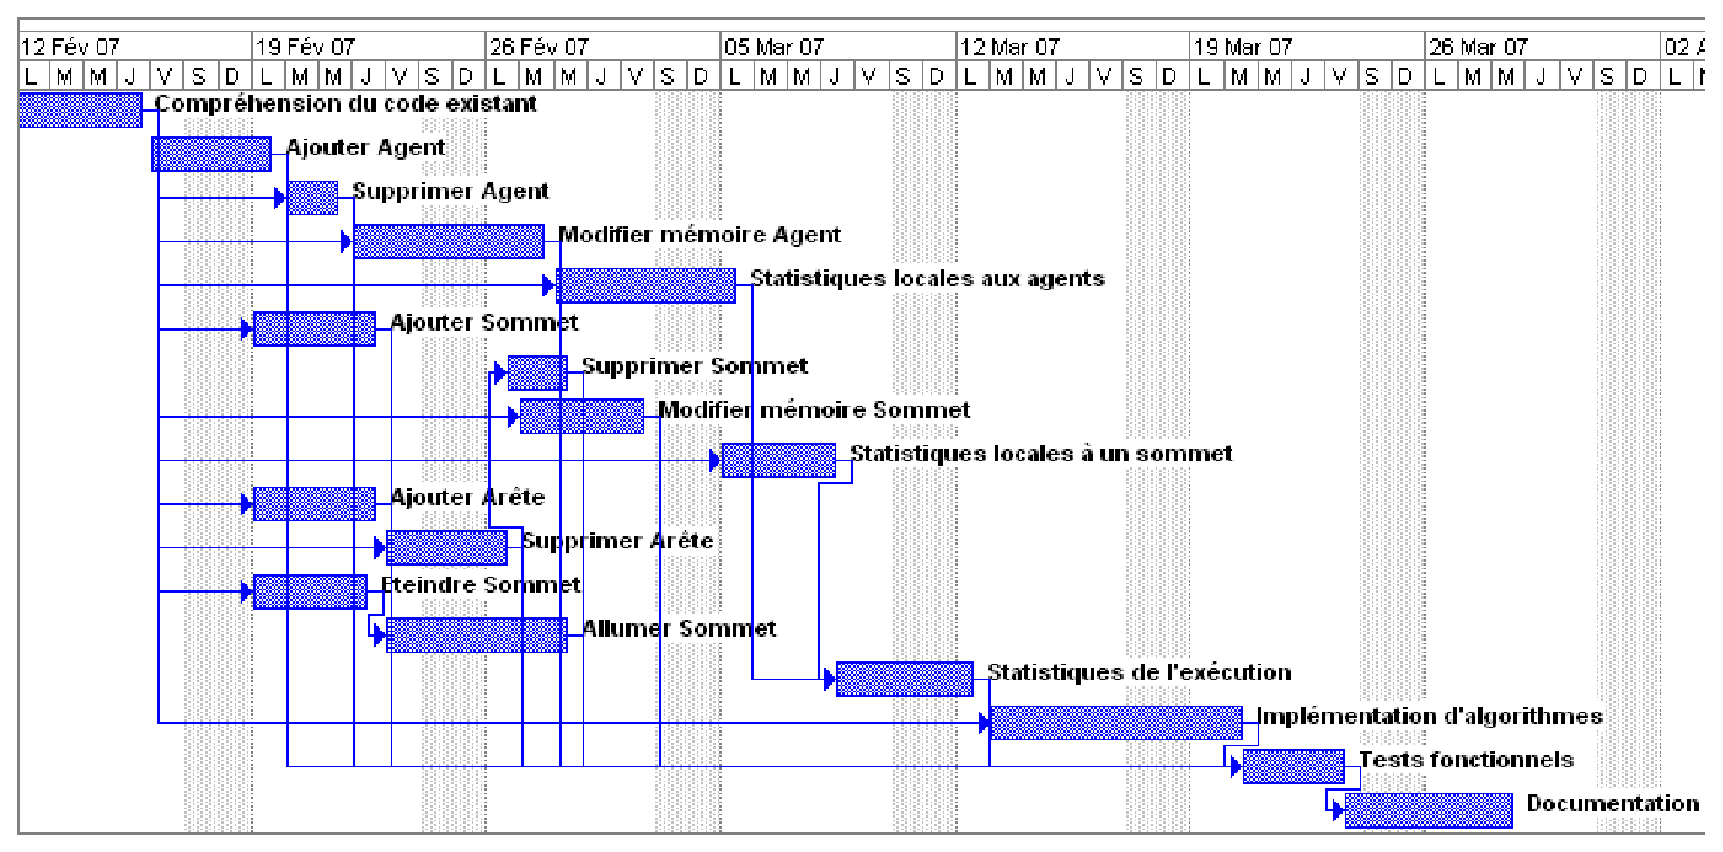
\includegraphics[angle=90,scale=0.8]{gantt}
  %\includegraphics[scale=0.8]{visidia.gantt}
  \caption{Diagramme de Gantt}
  \label{fig:gantt}
\end{figure}


L'�quipe  des r�alisateurs rencontrera  les clients  une fois  par semaine
pour faire le point sur le travail effectu�. L'horaire du vendredi matin �
10h  a �t� retenu  pour cette  entrevue hebdomadaire.  Les clients  et les
r�alisateurs resteront  en contact et  pourront �changer sur le  projet au
moyen d'une liste de diffusion \ref{mailing-list}.

Un diagramme  de Gantt \ref{fig:gantt}  planifie les grandes �tapes  de la
r�alisation du projet. Ce diagramme sera mis � jour au cours de la vie du projet.

\section{�ch�ancier}

La date de remise des rapports de fin de PFA aux clients est fix�e au
vendredi 14 avril, 17h00 derni�re limite.

La remise du projet donnera lieu � une soutenance dont la date est
fix�e au jeudi 27 avril.

%\section{Description des outils}
%% - D�ploiement (cd,dvd,autre)
%% - Presentation du portail, du site, de la mailing liste, etc.
%% - methode de validation du travail (tests, iteratif ou unitaire)

%\section{Utilisation d'une plate-forme de d�veloppement}
\section{Plate-forme de d�veloppement}

Le projet sera l'occasion d'utiliser un portail �volu� de
d�veloppement sur le mod�le du c�l�bre portail
%\href{http://sourceforge.net}{SourceForge}.
%\url{http://sourceforge.net} 
SourceForge \cite{SourceForge}.
Notre choix s'est port� sur le portail
%\href{http://www.berlios.de}{\berlios}
%\url{http://www.berlios.de} 
\berlios \cite{BerliOs} pour des raisons de rapidit� des
serveurs. Notre projet \visidia dispose ainsi d'une page d'accueil \cite{visidiaPFA}.\\
\url{http://visidia.berlios.de}\\
%\href{http://visidia.berlios.de}{\visidia.\berlios} 

%% \begin{verbatim}
%% http://visidia.berlios.de
%% \end{verbatim}

Cette page  d'accueil est un  wiki \cite{wiki}. Cela permet  une �volution
plus souple des informations pr�sent�es. Cette page est le point de d�part
vers  les  diff�rents services  fournis  par  \berlios.  Tous les  modules
d�crits par la suite peuvent �tre  retrouv�s � partir de la page d'accueil
du projet.\\

Tout d'abord les sources de notre extension de \visidia sont
maintenues gr�ce au gestionnaire de version Subversion
\cite{subversion}. Le client a la possibilit� de suivre l'avanc�e du
projet en acc�dant aux sources. Deux interfaces web permettent l'acc�s
aux sources: viewcvs \cite{viewcvs} et websvn \cite{websvn}.\\ 
%\href{http://svn.berlios.de/viewcvs/visidia/}{viewcvs}
\url{http://svn.berlios.de/viewcvs/visidia/}\\
%\href{http://svn.berlios.de/wsvn/visidia/}{websvn}
\url{http://svn.berlios.de/wsvn/visidia/}\\ 

Il est �galement possible de t�l�charger anonymement les sources
depuis le d�p�t Subversion:
\begin{verbatim}
svn checkout svn://svn.berlios.de/visidia/trunk
\end{verbatim}

L'�quipe  a aussi mis  en place  des mailing-lists  g�r�es par  le portail
\berlios.   Une  mailing-list  permet  aux  clients de  joindre  tous  les
r�alisateurs  et vice  versa. L'adresse  de cette  liste de  diffusion est
%\url{mailto:visidia-pfa@berlios.de}
\label{mailing-list}:
\begin{verbatim}
visidia-pfa@berlios.de
\end{verbatim}

Il est possible  de consulter les archives de cette  liste de diffusion au
moyen d'une interface web \cite{mailing-list}.\\
\url{https://lists.berlios.de/mailman/private/visidia-pfa/} 
 

%% Local Variables:
%% mode: latex
%% coding: latin-1
%% TeX-master: "main"
%% End:

\chapter*{Conclusion}
\addcontentsline{toc}{chapter}{Conclusion}
Les fonctionnalit�s demand�es par le client dans le cahier des charges ont �t�
toutes d�velopp�es. Nous avons �galement r�ussi � impl�menter le nombre voulu
d'algorithmes. Nous avons aussi, dans la mesure possible, essay� de d�velopper les
fonctionnalit�s suppl�mentaires souhait�es. N�anmoins, une documentation plus
fournie aurait facilit� la compr�hension du code. Nous avons donc pr�t� une
attention particuli�re � la documentation du travail que nous avons r�alis�.\\

Ce projet a �t� l'occasion de pouvoir approfondir nos connaissances en java,
et plus particuli�rement les fonctionnalit�s d'acc�s concurent et de gestion
des threads. 
L'impl�mentation des agents nous a confront� � des situations de calcul
distribu� complexe o� l'information connue se limite � celle de l'agent et du
sommet o� il se trouve.
L'exercice de reprise de code existant a �t� difficile � appr�hender. Il nous a
�t� toutefois b�n�fique d'y �tre confront� car nous seront s�rement amen� � le
rencontrer souvent en entreprise.\\

L'algorithmique distribu� �tant de plus en plus utilis� dans les syst�mes
informatique, ce projet a �t� l'occasion d'acqu�rir une exp�rience sur cette technologie.


\chapter*{Annexe}
\addcontentsline{toc}{chapter}{Annexe}
  %\input{algorithmes}

\end{document}
